\documentclass[11pt,a4paper]{article}
\usepackage[margin=25mm]{geometry}
\usepackage[T1]{fontenc}
\usepackage[utf8]{inputenc}
\usepackage{mathptmx,amsmath,amssymb,microtype,graphicx,booktabs,tabularx,array}
\usepackage[font=small,labelfont=bf]{caption}
\usepackage{tikz}
\usetikzlibrary{arrows.meta,positioning}
\usepackage[hidelinks]{hyperref}
\hypersetup{pdfauthor={Panagiotis Vionis},pdftitle={RecChain: auditable renewable energy certificate issuance with calibrated screening}}
\usepackage{url}
\usepackage{flafter}
\setlength{\parindent}{1.2em}
\setlength{\parskip}{2pt}
\setlength{\emergencystretch}{3em}
\hyphenpenalty=10000
\exhyphenpenalty=10000
\widowpenalty=10000
\clubpenalty=10000
\displaywidowpenalty=10000
\renewcommand{\arraystretch}{1.12}
\newcolumntype{Y}{>{\raggedright\arraybackslash}X}
\newcommand{\code}[1]{\texttt{\small #1}}
\title{RecChain: auditable renewable energy certificate issuance with calibrated screening}
\author{Panagiotis Vionis\thanks{Corresponding author: \texttt{p.vionis@office365.uop.gr}.}\\[5pt]
\small Department of Business Administration and Organization\\
\small Business Intelligence and Analytics Laboratory, University of Peloponnese\\
\small Antikalamos, GR24100, Greece}
\date{}
\begin{document}
\maketitle
\begin{abstract}
RecChain is an Ethereum prototype for screening reported renewable generation before certificate issuance. The system checks workflow identity, prevents repeated issuance for a registered meter interval, and stores hashes of the reading, reference history and screening policy. These records allow later review of the decision when the corresponding input data are available. Three admission policies are evaluated on public data from three photovoltaic installations. A capacity limit alone is compared with the same limit combined with either a rolling z score or an exponentially weighted residual. The weighted rule is calibrated on earlier data, and its threshold remains fixed during testing. Earlier corrupted readings can enter subsequent reference histories. At 1\% attempted corruption, the weighted rule gives mean F1 of 0.441, 0.108 and 0.175 across the sites. The corresponding values for the rolling rule are 0.405, 0.138 and 0.277. The comparison also measures excess energy admitted and unmodified energy withheld. These outcomes show how threshold selection affects the volume available for certification. Local execution gas averages approximately 426,000 for a report containing one meter and 1.13 million for a report containing three meters, excluding oracle and transport charges. The evaluation combines controlled changes to public generation records with local contract tests and workflow compilation.
\end{abstract}
\noindent\textbf{Keywords:} Renewable energy certificates; blockchain; decentralised oracles; anomaly detection; threshold calibration; smart contracts.


\section{Introduction}
A renewable energy certificate (REC) conveys the environmental attributes associated with one megawatt hour of eligible renewable electricity generation. Issuance, transfer and retirement within a recognised tracking system establish who may claim those attributes \cite{epa}. Guarantees of Origin serve a related role in European electricity markets, subject to their own eligibility and reporting rules. A digital token can record ownership of these attributes, while verification of the underlying generation remains the responsibility of meter and registry controls.

Blockchain provides a shared transaction record and rules for managing certificate balances. At the boundary between a physical installation and the registry, the reliability of the source data remains a separate concern. A contract can enforce conditions on a reported reading. Its ability to assess that reading depends on the information supplied by the meter interface and oracle service. Agreement among oracle nodes establishes consistency of their response, but the physical measurement still requires independent assurance.

RecChain places a screening step before issuance. An oracle retrieves a production reading and its history, calculates a residual score and forwards an accepted quantity to the registry. Rejected readings are withheld from this issuance path and can be reviewed. The prototype also retains a separate manual path for authorised issuers.

The work follows the review of blockchain applications in energy \cite{review} and the comparison of REC implementations on Solana and Ethereum \cite{comparison}. The latter examined transaction time and fees and identified automated verification of production data as a direction for further work. Ethereum is retained here to use the existing application and EVM tools.

The study examines the connection between screening and certificate issuance. Fu et al.\ \cite{fu} demonstrated issuance through blockchain oracles and divisible certificates, while Haryani et al.\ \cite{haryani} implemented a semifungible ERC1155 model. RecChain records the production interval and commitments to the evidence and policy used for each workflow decision. Its evaluation compares thresholds fitted on earlier observations with later public installation data, including histories affected by preceding corruptions. Measuring energy admitted and withheld shows the consequences of these choices for certificate volume. The contribution is the implementation and evaluation of this admission process using established statistical tools.

\section{Related work}
Blockchain certificate systems address transaction traceability, divisibility and settlement in different ways. Zuo \cite{zuo} describes a token based platform for REC issuance, trading, verification and retirement. Fu et al.\ \cite{fu} use blockchain oracles to retrieve production data and issue divisible certificates, including kWh level representation. Haryani et al.\ \cite{haryani} adopt ERC1155 semifungible tokens in a prototype for the Indonesian grid. Cali et al.\ \cite{cali} examine cybersecurity and adoption considerations in a token based REC framework. These systems provide the basis for examining how a screening policy affects issuance.

ERC1155 associates separate balances and metadata with multiple token identifiers in one contract \cite{erc1155}. This suits a batch model in which units from one production batch are interchangeable while attributes differ between batches. ERC20 can also support batch separation through additional contracts or application logic, and ERC721 can be extended to support fractional ownership. ERC1155 provides these batch balances within the contract used here.

Recent systems also check plausibility before ledger entry. The SolarChain preprint \cite{solarchain} uses meteorological and geometric constraints on photovoltaic output. WindChain \cite{windchain} checks wind resource claims using physical admissibility and an epoch level gate; its resource attestation problem differs from settlement against metered generation. RecChain examines a complementary question: how a historical statistical policy behaves when earlier corruptions enter its reference data, and how its decisions are recorded by the issuance contract.

Table~\ref{tab:related} compares the mechanisms reported in the closest publications. The comparison is limited to those research implementations. Statutory registries also apply institutional controls, and a publication may omit procedures used outside its reported experiment.

\begin{table}[tb]\centering\small
\caption{Closest research systems and the scope of their reported validation. No cross study accuracy ranking is implied.}\label{tab:related}
\begin{tabularx}{\linewidth}{@{}p{29mm}YY@{}}\toprule
System & Certificate or energy mechanism & Validation relevant to this study\\\midrule
Fu et al.\ \cite{fu} & Oracle mediated divisible certificates & Statistical screening experiment not reported\\
Haryani et al.\ \cite{haryani} & ERC1155 certificate prototype & Statistical screening experiment not reported\\
SolarChain \cite{solarchain} & Solar credits and market mechanisms & Physics based upper bound before ledger entry; preprint\\
WindChain \cite{windchain} & Wind resource provenance & Physical admissibility and epoch constraints on resource claims\\
RecChain & ERC1155 issuance with interval and evidence records & Frozen thresholds, received data histories and energy consequences on three PV sites; local contract tests\\\bottomrule
\end{tabularx}\end{table}


Statistical rules provide interpretable anomaly scores with modest computational requirements. Reviews of IoT anomaly detection \cite{fahim,nassif} cover these methods alongside learned models, while Munir et al.\ \cite{munir} compare traditional and deep methods on streaming data. Their relative performance depends on the data, feature representation and evaluation setting. Controlled anomaly injection is used because verified REC meter fraud labels are unavailable for the data examined here.

I compare a rolling z score with a robust median/MAD score, a Tukey fence score, an exponentially weighted residual score and an isolation forest \cite{tukey,isolation}. The weighted score is related to EWMA monitoring \cite{montgomery}, but its denominator and threshold differ from those of a classical EWMA control chart. A rule used before issuance must also be assessed through the consequences of its selected threshold.

Oracle design separates the acquisition of external data from the consensus that delivers a result to the contract \cite{chainlink2,pasdar}. RecChain places the screen within this acquisition and computation path. Its security still depends on the reporting interface, workflow configuration and receiving contract. Statistical consistency can identify an unusual report, whereas meter authentication and interval level uniqueness require separate controls.

\section{RecChain architecture and issuance}
\subsection{System and certificate lifecycle}
RecChain comprises a meter facing interface, an EVM registry, an application service and a web interface. The meter interface exposes production readings over HTTP. The registry records certificate batches, balances, listings and retirements. An Express service reads contract state, supports monitoring and generates certificate documents. A React/Vite interface provides issuance, portfolio, marketplace and public verification views. Wallet transactions may interact directly with the contract, while document generation depends on the application service.

The original integration uses Chainlink Functions. An authorised issuer requests a reading; the oracle runs a configured script and returns a result to the registry callback. Chainlink deprecated Functions on 15 June 2026 for testnets and 30 June 2026 for mainnet \cite{functions}. The replacement uses a Chainlink Runtime Environment (CRE) workflow and a receiving contract. Figure~\ref{fig:architecture} distinguishes these paths and the evidence available for each.

\begin{figure}[tb]
\centering
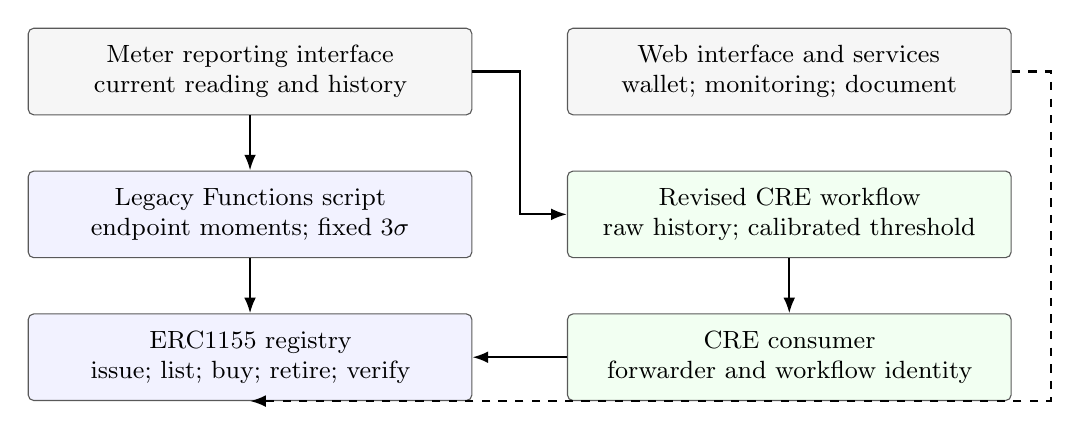
\begin{tikzpicture}[node distance=7mm,box/.style={draw=black!65,rounded corners=2pt,align=center,font=\small,minimum height=11mm,text width=54mm},flow/.style={-{Latex[length=2mm]},thick}]
\node[box,fill=gray!7] (meter) {Meter reporting interface\\current reading and history};
\node[box,fill=gray!7,right=12mm of meter] (ui) {Web interface and services\\wallet; monitoring; document};
\node[box,fill=blue!5,below=of meter] (legacy) {Legacy Functions script\\endpoint moments; fixed $3\sigma$};
\node[box,fill=green!5,below=of ui] (cre) {Revised CRE workflow\\raw history; calibrated threshold};
\node[box,fill=green!5,below=of cre] (consumer) {CRE consumer\\forwarder and workflow identity};
\node[box,fill=blue!5,below=of legacy] (registry) {ERC1155 registry\\issue; list; buy; retire; verify};
\draw[flow] (meter)--(legacy);
\draw[flow] (meter.east) -- ++(6mm,0) |- (cre.west);
\draw[flow] (legacy)--(registry);
\draw[flow] (cre)--(consumer);
\draw[flow] (consumer)--(registry);
\draw[flow,dashed] (ui.east) -- ++(5mm,0) |- (registry.south);
\end{tikzpicture}
\caption{RecChain components. The Functions path was deployed on Sepolia. The current CRE revision is tested locally and compiles to WASM; it has no live CRE deployment. Dashed routing denotes application or direct wallet access. The consumer checks the forwarder and pinned workflow metadata.}\label{fig:architecture}
\end{figure}

The five meter installations in the application are simulated. Consequently, the deployment demonstrates software integration rather than a connection to physical revenue meters. The national generation and public PV installation series evaluated below are separate screening experiments. They are not live inputs from these simulated installations.



One ERC1155 identifier represents one production batch and one token unit represents one kWh. A 35 MWh batch therefore contains 35,000 units under one identifier. The issuance floor is 1,000 kWh; fractional operation below one MWh applies to transfer and retirement rather than to the creation of a new batch. The selected unit size is an implementation parameter and does not establish that fractional claims are accepted by a certificate scheme.

The registry supports issuance through \code{issueRec}, escrow listing through \code{listRec}, ETH settled purchase through \code{buyRec}, and retirement through \code{retireRec}. Retirement burns the selected units and records the retiring account and quantity. A batch becomes fully retired when cumulative retirement reaches its issued volume. Each batch carries producer and issuer addresses, an energy source category, location, issued quantity, issuance time, expiry time and a provenance reference. Expiry is set to 365 days after issuance as a prototype policy, rather than as a claim about all REC or Guarantee of Origin schemes.

The \code{ISSUER\_ROLE} permits manual issuance and legacy oracle requests. The administrator assigns roles and configures the oracle path. Manual issuance stores the calling account as issuer and accepts a supplied provenance reference. Legacy oracle issuance records the registry address, while the revised workflow registry records its consumer. Issuer addresses can therefore distinguish the intended issuance paths. A string beginning with \code{oracle://} or \code{cre://} is not itself evidence that screening occurred, since a manual issuer may supply an arbitrary string.

Burning prevents reuse of the same retired token balance. The workflow path adds interval consumption for each governed meter identifier, as described below. Manual and legacy requests retain separate issuance authority, and no external registry reconciles the underlying generation. The prototype therefore provides local workflow interval controls and token balance accounting rather than a general guarantee against duplicate environmental claims.

\subsection{Screening and issuance controls}
An issuer calls \code{requestAutoIssuance}, which stores the production attributes against a request identifier. The Functions script retrieves a reading and rejects invalid, nonnumeric or negative values and values above 100 GWh. It also rejects when
\begin{equation}\left|\frac{x-\widehat\mu}{\widehat\sigma}\right|>3,\label{eq:legacy}\end{equation}
where the endpoint supplies both the current quantity $x$ and the reference moments. A successful callback mints only when the returned volume meets the one MWh floor. A response below the issuance floor terminates without minting and, in the legacy implementation, without an explicit outcome event.

Equation~\eqref{eq:legacy} describes a gate whose baseline is supplied by the endpoint. It is not equivalent to independently reconstructing the trailing window used in the detector experiments. Moreover, the script skips this statistical test when the reference moments are absent. An endpoint controller can supply a consistent reading and moments, or omit the moments, without the statistical rule establishing their truthfulness. The detector results below therefore characterise independently calculated scores, rather than validate the security of the legacy gate.


The CRE implementation replaces this earlier path with a check of the raw reference history.


The workflow in \code{cre/screening/main.ts} obtains the current reading and history through HTTP, uses identical response aggregation, and applies the shared rule in \code{rule.ts}. Missing responses, invalid numbers, future or stale current timestamps, repeated historical timestamps, and histories containing the current or a later reading cause rejection. Current intervals end at an aligned UTC hour. The reference comprises the latest 30 finite same hour observations within 45 days, sorted chronologically. Insufficient history causes rejection. A configured capacity bound precedes the residual test. Threshold and capacity overrides can be supplied per meter; sample configuration values are examples, not calibrated operating recommendations.

An admitted report contains the canonical meter identifier, production start and end, integer kWh, an evidence hash and a policy hash. The evidence serialisation contains the current reading, selected timestamped history, residual score and rule version. The policy serialisation contains the threshold, weighting, window, quantity limits and freshness settings. The workflow computes Keccak256 commitments and logs the corresponding serialised receipts. An operator must retain and make these receipts available; the chain stores commitments, not the underlying data. A commitment permits a verifier with the receipt to check consistency with the recorded decision. Physical measurement accuracy and long term retention remain separate requirements.

The receiver requires the configured forwarder and a pinned workflow identifier, name and owner. The parser accepts the documented 64 byte metadata and a 62 byte packed test representation, validating the first 62 bytes in each case \cite{creconsumer}. DON report signature verification remains the forwarder's responsibility. Report consumption is scoped to the chain, consumer, workflow identifier and payload. Changing the two trailing report ID bytes cannot replay the same payload. The receiver checks meter binding, the 1 MWh floor and interval freshness, with a default maximum age of seven days. Invalid entries emit rejection events; a downstream registry failure reverts the transaction and its state changes.

The workflow registry stores the consumed interval and latest issued end for each governed meter identifier. Its key includes chain ID, registry address, meter hash and interval endpoints. Exact reuse is rejected even if the reported quantity changes. Requiring the next start to be at least the previous end also excludes overlap and out of order issuance. This state resides in the registry, so replacing the consumer or rotating the workflow identity does not reset it. Consumption state is set before the ERC1155 receiver hook, and the workflow entry point is guarded against reentrancy. Failed transactions roll back consumption, permitting a corrected retry.

These properties apply to the workflow entry path in one registry under canonical meter naming. A privileged manual or legacy issuer can still mint independently; registering aliases for the same physical meter or using another registry can also duplicate the underlying attributes. There is no reconciliation with an external tracking system. Sequential interval consumption can prevent later backfilling of a previously skipped interval. A correction procedure is therefore needed if historical backfilling is required.



The current reading and history originate from the same reporting interface. An adversary controlling it can fabricate a statistically consistent history. Oracle agreement establishes neither source truth nor device calibration. Interval consumption limits repeated workflow issuance from one governed identifier; it cannot establish that two different identifiers represent different installations. Hash commitments constrain later alteration of retained receipts without authenticating their initial contents.

The revision implements application level authorisation, history validation, replay guards and interval consumption. Device signatures, installation eligibility, independent meter trials, cross registry reconciliation and procedures for revocation remain outside its evidence. The local tests and compilation support the implemented control flow. They do not establish DON availability, report delivery latency or operation against authenticated physical meters.

\subsection{Certificate document and public verification}
The application generates a PDF document, termed a Carbon Passport, from registry metadata and retirement records. It includes the batch identifier, producer, source, location, quantities, dates, issuer address and provenance reference. A QR code opens a public page that reads contract state through an RPC provider. Readers can compare the document with ledger state without connecting a wallet, subject to the availability and accuracy of the hosted page and RPC service.

The document identifies the issuance path from the recorded issuer address. The revised registry also exposes the interval and the evidence and policy hashes through its receipt view and events. Checking these commitments requires the retained input receipt and an independent comparison. This operation has not yet been added to the document generator.

The \code{verifyRec} view reports whether a batch exists, remains partly unretired and has not expired. Assessment of a particular claim additionally requires the remaining balance, retirement quantity and the claimant's retirement record. Recognition by an external certificate registry is a separate requirement.

The displayed emissions conversion multiplies certificate volume by one European average grid factor. It is an illustrative grid equivalent. Market based Scope 2 accounting requires qualifying contractual instruments and applicable emission factors under the GHG Protocol \cite{scope2}. Avoided emissions require a defensible counterfactual. The displayed conversion establishes neither result. Conformity with GRI, ISO 14064, Part 1 or a statutory certificate scheme has not been demonstrated. The document serves as a research record of the prototype's ledger and retirement operations.

\section{Evaluation design}
\subsection{Screening methods}
For each current reading $x_t$, the reference window contains 30 preceding observations at the same UTC hour. On the measured series, these are the previous 30 retained complete days; missing days can make the calendar span longer. Matching the hour reduces the effect of the photovoltaic diurnal cycle. Let $\widehat\mu_t$ and $\widehat\sigma_t$ be the window mean and sample standard deviation. The rolling score is
\begin{equation}s_t^{z}=\frac{|x_t-\widehat\mu_t|}{\max(\widehat\sigma_t,\epsilon)}.\label{eq:z}\end{equation}
The weighted score replaces only the reference mean:
\begin{align}
w_i&=\frac{\lambda(1-\lambda)^{29-i}}{\sum_{j=0}^{29}\lambda(1-\lambda)^{29-j}},\quad i=0,\ldots,29,\label{eq:weights}\\
\widetilde\mu_t&=\sum_{i=0}^{29}w_i x_{t-30+i},\qquad
s_t^{e}=\frac{|x_t-\widetilde\mu_t|}{\max(\widehat\sigma_t,\epsilon)}.\label{eq:ewma}
\end{align}
Here $\lambda\in(0,1)$ controls the weight of recent observations. The limiting case $\lambda\to0$ gives the flat mean, while $\lambda\to1$ gives the most recent same hour observation. I call Eq.~\eqref{eq:ewma} an EWMA residual score. It is not a classical EWMA control chart because the scale is the unweighted window standard deviation and the threshold is an empirical residual quantile.

The robust score uses the median and $1.4826$ times the median absolute deviation. The Tukey score is the distance beyond the interval $[Q_1-1.5\,\mathrm{IQR},Q_3+1.5\,\mathrm{IQR}]$, divided by the floored IQR. A negative Tukey score lies inside the fence. All four statistical rules use a dispersion floor $\epsilon=1$ in the native data units: kWh in the synthetic series and MW in the national generation extract. These units are not interchangeable. The measured series is retained as power at hourly resolution and is not presented as a rescaled installation level energy series.

For the statistical rules, solar observations below one native unit at night receive the lowest score. The synthetic definition uses its fixed daylight envelope; the measured definition uses solar elevation below $-6^\circ$ at $39^\circ$N, $22^\circ$E, corresponding to the end of civil twilight rather than astronomical twilight. The isolation forest uses 200 trees and the default maximum subsample size of 256. Synthetic features include quantity, hour, standardised residual and quantity to mean ratio; models are fitted by energy source. The measured experiment pools both sources and omits hour as a feature. Forest fitting uses the evaluation corpus without labels, so its results are transductive comparisons rather than evidence of a frozen deployed model.

\subsection{Synthetic and national generation experiments}\label{sec:chronological}
The synthetic fleet comprises two solar, two wind and one hydro meter. Each replication spans 180 days; the first 30 supply the initial history, leaving 18,000 evaluated readings. Solar generation has a half sine reference profile between 04:00 and 17:00 UTC, with peak at 10:30 UTC. Wind and hydro use sinusoidal multipliers with amplitudes 0.15 and 0.05. A source specific autoregressive daily multiplier, additive measurement noise and linear decay are then applied before nonnegative clipping. The detector estimates its baseline from observations rather than receiving the generator's parameters.

These are controlled profiles, not calibrated physical models. In particular, the daily decay coefficients in the released generator range from 0.0005 to 0.006 and produce changes much larger than ordinary annual equipment degradation. Additive noise can also produce nonzero solar readings outside the daylight envelope. The benchmark can compare scoring rules under its specified variation; it cannot estimate their accuracy on operational meters.

Anomaly attempts are assigned to 10\% of evaluation readings, sampled without replacement. Outside the solar daylight envelope, a selected solar reading is replaced with 200 to 500 kWh. Other selected readings receive one of five transformations with equal probability: a large upward displacement of 5 to 8 window standard deviations, a large downward displacement of the same size clipped at zero, a moderate upward displacement of 2.5 to 4.5 standard deviations, a collapse to 5 to 15\% of the original value, or a zero replacement. The collapse is not a frozen sensor sequence. An injection label records the attempted transformation, which may leave a value unchanged when it is already zero.

Reference windows are formed before injection. An earlier injected anomaly therefore never contaminates a later baseline, unlike operation with undetected erroneous readings. Thirty replications use seeds 1000 to 1029. Mean metrics are accompanied by $1.96$ times their standard error across replications. These intervals describe simulation variability under the chosen generator and should not be read as uncertainty over physical installations.


The national generation experiment uses a separate measured series.


The measured experiment uses the Open Power System Data release of 6 October 2020, which republishes national generation from the transparency platform operated by the European Network of Transmission System Operators for Electricity \cite{opsd}. The Greek solar and onshore wind extract spans January 2018 to September 2020 and contains 24,070 hourly records. Retaining complete days leaves 1,000 days for each source. After the 30 observation warm up, each source contributes 23,280 current reading/window pairs, giving 46,560 pairs in total. These national aggregates capture weather and reporting variation, but they do not validate the behaviour of individual revenue meters.

The measured data generator differs from the synthetic generator in more than the normal series. Night time injection replaces a solar reading with 5 to 20\% of a source capacity proxy. Non night injection selects four categories with equal probability: large spike, large dropout, moderate spike and low output collapse. There is no separate zero replacement category in this experiment, although downward displacement can produce zero through clipping. The measured results therefore concern this four category protocol rather than an identical replication of the synthetic injection model.

In the archived whole series experiment, the capacity proxy is the larger of the window maximum and the source's whole series 99th percentile. Its use of later observations affects injection magnitudes, including anomalies in the earlier partition. It is not a detector feature, but it prevents describing the complete simulation procedure as prospectively isolated. The chronological evaluation below instead estimates this source percentile from calibration data only.

Prevalence is varied over 0.5\%, 1\%, 5\% and 10\%, with seeds 2000 to 2029. For the retrospective matched budget comparison, each detector's threshold is the empirical $(1-p)$ quantile of its evaluation scores, where $p$ is the injected prevalence. This uses the test score distribution and assumes knowledge of prevalence. It is useful for comparing rankings at a prescribed alarm volume, but it is not an operational thresholding policy. Quantiles are estimated from finite scores; ties and the exclusion of night time $-\infty$ scores from the Tukey quantile can prevent exact matching of alarm counts. Precision and recall coincide only when the number of alarms equals the number of injected labels.

The fixed threshold comparison uses 2.5 for the standardised statistical scores and the conventional fence for Tukey. The isolation forest has no corresponding sigma scale, so its matched budget result is repeated for reference and is explicitly marked as such. The gate deployed in the legacy oracle uses $3\sigma$, whereas 2.5 is the monitoring threshold used for this comparison. Neither fixed threshold is calibrated to a known false positive probability under these data.


A further chronological comparison fits thresholds on an earlier period and then keeps them fixed.


The earlier 40\% of retained evaluation days, before 23 February 2019, provide 18,624 calibration observations; the remaining days provide 27,936 test observations. Prior same hour readings may initialise test windows because they would be available when the current reading is scored. Windows continue to use the unmodified series, so this remains a conditional experiment with uncontaminated historical baselines.

I select $\lambda$ from $\{0.05,0.1,0.2,0.3,0.5,0.7,0.9\}$ by mean calibration F1 over twelve injection seeds at 1\% prevalence and a calibration only matched budget. The source capacity percentile is calculated on the calibration observations only. Injection is performed separately within each partition, preserving the four non night categories of the released measured generator. The selected value is $\lambda=0.5$, with calibration F1 of 0.560; the values at 0.05 and 0.9 are 0.520 and 0.541. This parameter selection is conditional on the injection model and does not identify a general optimum for REC meters.

Thresholds are then calculated from the \emph{unmodified} calibration scores at nominal alert rates of 1\%, 0.5\% and 0.1\%. No score quantile is fitted on the test partition. I first measure their alert rates on the unmodified test series, then evaluate injected test anomalies over seeds 5000 to 5011 with thresholds calibrated to 1\% and then held fixed. The latter distinguishes ranking performance from an implementable thresholding procedure. Natural anomalies in the unmodified data are unknown; hence these empirical historical alert rates are not measured false positive rates.

\subsection{PV installation experiment}\label{sec:sites}
The PVDAQ Public Datasets provide installation level photovoltaic output and hardware metadata \cite{pvdaq}. I use the public system snapshot dated 29 July 2025. Before fitting detectors, systems are sorted by numeric identifier and filtered to reported quality status ``pass'', at least two years of data and at least 10 kW DC capacity. The first system in each distinct K\"oppen climate class is selected, stopping at three. This deterministic rule gives systems 34, 1199 and 1239 (Table~\ref{tab:sites}). It does not produce a representative sample of PV installations.

Initial inspection of the 2018 daily files found an August change in channel scale at systems 34 and 1239 and disappearance of the aggregate AC channel at system 1199. Applying one annual conversion would introduce artificial anomalies. Before any detector result was calculated, the common evaluation period was restricted to January to July, the last full month preceding the discontinuity. This amendment is recorded in the supplied protocol. No magnitude based repair of the later values is attempted. Pre August conversion factors from the metric metadata are 0.1, 0.001 and 1.0 kW per raw channel unit for systems 34, 1199 and 1239, respectively.

Timestamps are interpreted in the supplied IANA time zones and converted to UTC. Ambiguous or nonexistent local times are excluded. Duplicate timestamps, if present, are averaged. Negative net values are clipped to zero, and samples exceeding 1.2 times DC nameplate power are excluded by a common quality rule. No sample exceeds that bound in the retained period. The median observed cadence, rounded to a minute, is 15, 5 and 15 minutes. Rectangular integration approximates hourly kWh; an hour requires 75 to 125\% of the expected sample count. Hour labels denote UTC interval ends. Missing hours remain missing, including absent night records at system 1199. These are approximations from sampled AC power, not certified revenue meter energy registers.

\begin{table}[tb]\centering\small
\caption{PVDAQ sites and retained UTC hourly records, January to July 2018. Thresholds use calibration only. Climate codes follow the public system metadata.}\label{tab:sites}
\begin{tabular}{@{}lrrrrr@{}}\toprule
System (climate) & DC kW & Finite hours & Calibration & Test & EWMA threshold\\\midrule
34 (Bwh) & 146.64 & 5,066 & 1,815 & 2,531 & 3.225\\
1199 (Cfa) & 52.92 & 2,654 & 765 & 1,436 & 3.151\\
1239 (Dfb) & 20.16 & 5,079 & 1,818 & 2,541 & 3.493\\
\bottomrule\end{tabular}\end{table}


The first 106 calendar days, before 17 April 2018 UTC, form calibration; the remaining 106 days form testing. Each eligible reading requires 30 finite prior observations at the same UTC hour within 45 calendar days. Earlier data may initialise a later window, but current and future readings cannot enter it. The resulting calibration and test counts are 4,398 and 6,508. The common time interval and missing data rules apply identically to all policies.



All policies reject current hourly energy above 1.2 times the site's DC capacity expressed as one hour energy. The first policy uses only this capacity guard. The second adds Eq.~\eqref{eq:z} at a fixed threshold of 3. The third adds Eq.~\eqref{eq:ewma}, with $\lambda=0.5$ fixed from the national generation experiment, and a separate threshold equal to each site's 99th calibration score percentile. All scores use $\epsilon=1$ kWh. No test quantile or injected test label adjusts a threshold. A site specific threshold provides an operating comparison with the fixed rolling rule, not a controlled comparison of weighting alone.

Interventions affect 1\% or 5\% of eligible test readings, sampled without replacement for seeds 6000 to 6011. For non night readings, five equally probable transformations are 50\% over reporting, 150\% over reporting, 50\% under reporting, replacement with zero, and collapse to 5 to 15\% of the unmodified value. Night is approximated from solar elevation below $-6^\circ$ at the site coordinates and the UTC hour. A selected night reading is replaced with 5 to 20\% of DC capacity as one hour ghost energy. Magnitudes do not depend on a detector's window standard deviation. If a transformation leaves the value unchanged, it is excluded from positive labels. Realised positive rates are therefore slightly lower than the attempted rates.

Two causal history modes are retained. In the diagnostic mode, windows use the unmodified series. In the received history stress test, every received value, including earlier injected and flagged values, enters later windows when its timestamp is selected. This tests contamination rather than a cleansing policy; no result dependent repair is applied. The deployed history validator can reject malformed or incomplete responses independently of the scoring experiment. Results below emphasise received history, while both modes and every seed are supplied.

For positive labels defined only by the interventions, I report precision, recall and F1. Unmodified readings can contain natural faults, so alarms on them are not verified false positives. Let $x_t$ be the unmodified value, $v_t$ the received value, $y_t$ the intervention label and $A_t\in\{0,1\}$ the admission decision. Energy consequences are
\begin{align}
 E_{\mathrm{excess}}&=\sum_t A_t\max(v_t-x_t,0),\\
 E_{\mathrm{withheld}}&=\sum_t (1-A_t)(1-y_t)x_t.
\end{align}
The fraction of excess energy rejected divides the excluded positive differences by their total. Withheld unmodified energy is divided by the total energy of unmodified readings. These metrics distinguish missed over reporting from the withholding of reference output. Means and Student $t_{11}$ confidence half widths describe variation over twelve intervention seeds conditional on the fixed sites and periods.

The PV sites produce less than 1 MWh in an hour, so their screened hourly records are not minted by the present hourly workflow. Monthly sums and the 1 MWh floor are computed only as analytical batch equivalents. The prototype does not yet implement an accumulator that commits all screened sub MWh intervals into a monthly certificate. Consequently, the measured data experiment validates a screening policy; the separate contract experiments validate issuance from supplied report fixtures. This separation prevents presenting the study as an end to end physical deployment.

\section{Results and discussion}
\subsection{Synthetic and national generation results}
Table~\ref{tab:synthetic} reports the archived synthetic results at the matched retrospective budget. The weighted and rolling scores have similar F1, with mean values 0.831 and 0.826. This difference is small relative to the distinction between those methods and the median/MAD rule under the chosen generator. Because corruption magnitudes depend on the window standard deviation, the injection model also aligns with the scale used by the two leading scores. Their ranking is therefore conditional on that model rather than evidence of general superiority.

\begin{table}[tb]\centering\small
\caption{Synthetic results over 30 replications of 18,000 readings. Entries are mean $\pm$ 95\% normal confidence half width. Thresholds are fitted retrospectively to a nominal 10\% alarm budget.}\label{tab:synthetic}
\begin{tabular}{@{}lccc@{}}\toprule
Detector & Precision & Recall & F1\\\midrule
EWMA residual & $0.831\pm0.003$ & $0.831\pm0.003$ & $0.831\pm0.003$\\
Rolling z score & $0.826\pm0.003$ & $0.826\pm0.003$ & $0.826\pm0.003$\\
Isolation forest & $0.806\pm0.003$ & $0.806\pm0.003$ & $0.806\pm0.003$\\
Tukey fence & $0.828\pm0.003$ & $0.765\pm0.003$ & $0.795\pm0.003$\\
Median/MAD & $0.454\pm0.007$ & $0.454\pm0.007$ & $0.454\pm0.007$\\\bottomrule
\end{tabular}
\end{table}

The Friedman aligned ranks comparison treats seeds as paired blocks, subtracts the mean within each block and jointly ranks the aligned observations \cite{garcia}. Applied to the per seed F1 values, it gives $T=110.50$, with four degrees of freedom and $p=5.69\times10^{-23}$. Table~\ref{tab:ranks} gives the mean aligned ranks and Finner adjusted comparisons against the weighted score control. The comparison does not reject equality between the weighted and rolling scores, and failure to reject does not establish equivalence. Comparisons against a control do not establish every pairwise ordering.

\begin{table}[tb]\centering\small
\caption{F1 aligned ranks analysis on the synthetic benchmark. Lower rank is better. Finner adjusted $p$ values compare each method with the best ranked control \cite{finner}.}\label{tab:ranks}
\begin{tabular}{@{}lrr@{}}\toprule
Detector & Mean aligned rank & Adjusted $p$\\\midrule
EWMA residual & 22.10 & Control\\
Rolling z score & 39.17 & 0.128\\
Isolation forest & 79.17 & $4.84\times10^{-7}$\\
Tukey fence & 101.57 & $2.80\times10^{-12}$\\
Median/MAD & 135.50 & $2.01\times10^{-23}$\\\bottomrule
\end{tabular}
\end{table}

For the rolling score, the fixed threshold sweep gives its largest synthetic F1 at $|z|\geq3$. Recall decreases from 0.901 at threshold 2 to 0.646 at threshold 4. This observation does not validate the legacy issuance gate: its moments originate from the endpoint, the synthetic prevalence is fixed at 10\%, and the whole series threshold sweep is retrospective. At the 2.5 monitoring threshold, large spikes are detected in 99.7\% of attempts, compared with 73.9\% for moderate spikes and 65.7\% for night generation injection. The more difficult categories are therefore not resolved by the high overall ranking of the score.



Table~\ref{tab:measured} reproduces the archived F1 values on the measured series under the actual injection protocol. At a matched budget, the weighted score is ahead of the rolling score at every evaluated prevalence. The fixed threshold produces much lower F1 at low prevalence for both. For example, at 1\% prevalence the rolling score changes from 0.518 under the matched budget to 0.277 at 2.5. This difference demonstrates sensitivity to the operating rule; it does not show that a deployment can recover the matched budget value without knowing the prevalence and test score quantile.

\begin{table}[tb]\centering\small
\caption{Archived measured series F1, averaged over 30 injection replications. Normal 95\% confidence half widths are below 0.014. Matched budget thresholds use test scores. The repeated forest values in the fixed block are still matched budget results.}\label{tab:measured}
\begin{tabular}{@{}lrrrrrrrr@{}}\toprule
 & \multicolumn{4}{c}{Retrospective matched budget} & \multicolumn{4}{c}{Fixed statistical threshold}\\
\cmidrule(lr){2-5}\cmidrule(l){6-9}
Injected prevalence & 0.5\% & 1\% & 5\% & 10\% & 0.5\% & 1\% & 5\% & 10\%\\\midrule
EWMA residual & .496&.551&.661&.716&.224&.351&.646&.722\\
Rolling z score & .470&.518&.624&.670&.169&.277&.584&.678\\
Isolation forest$^*$ & .431&.468&.582&.628&.431&.468&.582&.628\\
Tukey fence & .303&.355&.560&.631&.127&.217&.517&.625\\
Median/MAD & .284&.333&.533&.611&.091&.163&.455&.585\\\bottomrule
\end{tabular}
\par\smallskip\footnotesize $^*$No independently fixed forest threshold is evaluated in this table.
\end{table}

At 10\% prevalence, the rolling score F1 is 0.156 lower on measured data than on the synthetic benchmark. The two experiments differ in aggregation level, native units, night time injection and the sampled non night categories. Consequently, the gap cannot be attributed entirely to the replacement of synthetic normal readings by real readings. It indicates limited transferability of the synthetic estimate under these protocols, without quantifying a universal optimism correction for other studies.

The stored paired whole series comparisons favour the weighted score under matched budgets. Their uncertainty reflects only the locations and magnitudes of injected anomalies on the same measured series. Repeated injection does not create independent countries, installations or reporting periods. Statistical significance within that experiment cannot establish performance under different operational distributions.



A 30 observation window is insufficient for reliable nonparametric calibration of a 1\% or smaller tail. Interpolating an empirical quantile does not create additional tail observations. I therefore separate the short history used to calculate a residual from the longer corpus used to set its threshold. The 18,624 pooled calibration residuals support an empirical threshold, subject to serial dependence and differences between sources. They do not establish a per meter false rejection rate.

Table~\ref{tab:alerts} gives the thresholds and realised alerts on the unmodified test period. The absolute deviations from the targets are small in this split, but this does not establish general temporal stability. At the 0.1\% target, an observed rate near 0.07\% still represents a substantial relative difference, and the extreme tail contains relatively few effective observations. No confidence guarantee for future alert control follows without assumptions on dependence and distributional change.

\begin{table}[tb]\centering\small
\caption{Thresholds fitted on unmodified calibration scores and alert rates on the unmodified later period. The rates are empirical alerts, not verified false positive rates.}\label{tab:alerts}
\begin{tabular}{@{}lrrrr@{}}\toprule
 & \multicolumn{2}{c}{Rolling z score} & \multicolumn{2}{c}{EWMA, $\lambda=0.5$}\\
\cmidrule(lr){2-3}\cmidrule(l){4-5}
Nominal alert rate & Threshold & Test alerts & Threshold & Test alerts\\\midrule
1.0\% & 3.67 & 0.75\% & 2.95 & 1.09\%\\
0.5\% & 4.35 & 0.37\% & 3.48 & 0.56\%\\
0.1\% & 7.60 & 0.07\% & 7.37 & 0.07\%\\\bottomrule
\end{tabular}
\end{table}

Table~\ref{tab:frozen} then evaluates injected test anomalies using the frozen thresholds calibrated to 1\%. The weighted score has higher recall at every prevalence, but its precision is lower. At 0.5\% and 1\% prevalence its F1 is also lower than the rolling score. At 5\% and 10\% it has higher F1. This result qualifies the matched budget ranking: favouring recent observations improves sensitivity under this protocol, but the associated alarm burden can outweigh that gain when anomalies are infrequent.

\begin{table}[tb]\centering\small
\caption{Held-out detection with thresholds fitted to a nominal 1\% alert rate on unmodified calibration scores and then frozen. Entries are mean $\pm$ 95\% Student-t confidence half-width over twelve injection replications. Intervals condition on the same national series.}\label{tab:frozen}
\begin{tabular}{@{}lcccccc@{}}\toprule
 & \multicolumn{3}{c}{Rolling z-score, $\tau=3.67$} & \multicolumn{3}{c}{EWMA, $\lambda=0.5$, $\tau=2.95$}\\
\cmidrule(lr){2-4}\cmidrule(l){5-7}
Prevalence & Precision & Recall & F1 & Precision & Recall & F1\\\midrule
0.5\% & $0.273\pm0.009$ & $0.562\pm0.024$ & $0.367\pm0.013$ & $0.228\pm0.007$ & $0.646\pm0.026$ & $0.337\pm0.011$\\
1\% & $0.435\pm0.009$ & $0.571\pm0.021$ & $0.494\pm0.013$ & $0.376\pm0.007$ & $0.656\pm0.020$ & $0.478\pm0.011$\\
5\% & $0.798\pm0.003$ & $0.565\pm0.009$ & $0.662\pm0.007$ & $0.756\pm0.003$ & $0.650\pm0.010$ & $0.699\pm0.007$\\
10\% & $0.894\pm0.002$ & $0.569\pm0.006$ & $0.695\pm0.005$ & $0.869\pm0.001$ & $0.651\pm0.007$ & $0.744\pm0.005$\\
\bottomrule\end{tabular}
\end{table}


For a nominal historical alert target of 1\%, the frozen thresholds produce total alarm rates of 1.03\% for the rolling score and 1.41\% for the weighted score at 0.5\% injected prevalence. At 10\% prevalence those rates rise to 6.36\% and 7.49\%. An alert rate calibrated on unmodified history is not a hard cap after the data distribution changes or anomalies are added. Selecting a method for issuance therefore requires a policy for the cost of missed anomalies, delayed legitimate certificates and human review. The evidence supports retaining both scores as candidate operating rules rather than declaring the weighted statistic universally superior.

The chronological result concerns the statistical rule, not end to end oracle validation. The implementation rejects scores strictly above its threshold, while the evaluation convention includes equality. Moreover, the workflow must independently enforce the historical window assumptions before the test can represent its behaviour. No field claim is inferred from the numerical advantage of either detector.

\subsection{PV installation results}
\begin{table}[tb]\centering\small
\caption{F1 under received-data histories. Values are mean $\pm$ conditional 95\% confidence half-width over twelve intervention seeds. Rates denote attempted interventions, not verified fraud prevalence.}\label{tab:sitef1}
\begin{tabular}{@{}lrrrr@{}}\toprule
System & Rate & Capacity only & Rolling z & EWMA\\\midrule
34 & 1\% & $0.058\pm0.040$ & $0.405\pm0.031$ & $0.441\pm0.026$\\
34 & 5\% & $0.089\pm0.027$ & $0.683\pm0.022$ & $0.678\pm0.025$\\
1199 & 1\% & $0.078\pm0.044$ & $0.138\pm0.049$ & $0.108\pm0.057$\\
1199 & 5\% & $0.138\pm0.039$ & $0.227\pm0.044$ & $0.228\pm0.035$\\
1239 & 1\% & $0.077\pm0.040$ & $0.277\pm0.067$ & $0.175\pm0.059$\\
1239 & 5\% & $0.090\pm0.027$ & $0.283\pm0.028$ & $0.195\pm0.030$\\
\bottomrule\end{tabular}\end{table}

The ranking varies by site and intervention rate (Table~\ref{tab:sitef1}). At 1\%, the weighted rule has higher mean F1 at system 34, while the rolling rule is higher at systems 1199 and 1239. At 5\%, the two rules are close at systems 34 and 1199; the rolling rule remains higher at system 1239. These differences are descriptive, not tests of general superiority. Low recall at the latter two sites shows that rejecting the largest violations does not resolve the more moderate manipulations.

\begin{table}[tb]\centering\small
\caption{Received-history outcomes at 1\% attempted intervention. Energy columns are seed means; figure whiskers and the supplied replication results quantify uncertainty. Withheld energy excludes intervened readings.}\label{tab:siteenergy}
\begin{tabular}{@{}llrrrr@{}}\toprule
System & Policy & Recall & Excess admitted (kWh) & Excess rejected (\%) & Withheld (\%)\\\midrule
34 & Capacity only & 0.031 & 295.29 & 23.04 & 0.000\\
34 & Rolling z & 0.763 & 53.84 & 87.10 & 1.710\\
34 & EWMA & 0.741 & 52.61 & 87.39 & 1.263\\
1199 & Capacity only & 0.042 & 63.24 & 25.02 & 0.000\\
1199 & Rolling z & 0.095 & 49.07 & 40.58 & 0.016\\
1199 & EWMA & 0.089 & 52.26 & 36.75 & 0.054\\
1239 & Capacity only & 0.041 & 36.34 & 31.92 & 0.000\\
1239 & Rolling z & 0.165 & 23.96 & 55.55 & 0.000\\
1239 & EWMA & 0.099 & 28.68 & 46.42 & 0.002\\
\bottomrule\end{tabular}\end{table}

Table~\ref{tab:siteenergy} and Fig.~\ref{fig:siteenergy} show the operational tradeoff at 1\%. At system 34, either statistical rule excludes about 87\% of injected excess energy, against 23\% with capacity alone. The weighted rule withholds 1.26\% of unmodified energy, compared with 1.71\% for the rolling rule. At system 1199, the weighted rule excludes 36.75\% of excess energy and the rolling rule 40.58\%, while both withhold less than 0.1\% of reference energy. At system 1239, the corresponding exclusion fractions are 46.42\% and 55.55\%, with negligible withheld energy. These outcomes support local policy selection rather than a universal preference for the weighted rule.

\begin{figure}[tb]\centering
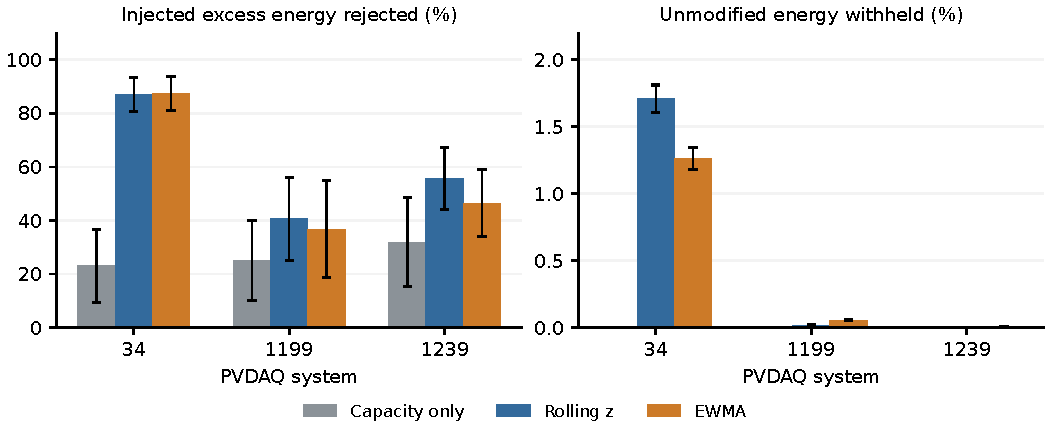
\includegraphics[width=\linewidth]{generated/site_energy.pdf}
\caption{Received history results at 1\% attempted corruption. Bars are seed means; whiskers are conditional 95\% confidence half widths. The panels use different vertical scales. Withholding concerns unmodified reference output, not verified legitimate generation.}\label{fig:siteenergy}
\end{figure}

Calibration to a historical alert target does not guarantee its later realisation. On the unmodified test period, weighted rule alert rates are 1.78\%, 0.56\% and 0\% at the three sites, despite the common nominal 1\% calibration target. Site seasonality, incomplete night coverage and the fixed 1 kWh scale floor affect the score distribution. The small sites also receive fewer interventions per replication. These limits explain why national aggregate rankings cannot be transferred directly to meter level operation.

\subsection{Local verification and execution cost}
The revised suite completes 72 Hardhat cases: 57 behavioural contract tests and fifteen gas harness cases. The shared screening rule completes ten unit tests, and the HTTP fixture exercise completes eight checks. Type checking and WASM compilation succeed. The contract tests cover forwarder and workflow identity, malformed metadata, payload replay with a changed report identifier, duplicate and overlapping intervals, consumer rotation, rollback on failure, access control, evidence records and expiry enforcement. These results are local verification, not a new security audit. Previously reported coverage and static analysis percentages are not reused as measurements of the revised code.

Purchase now rechecks expiry, and the ERC1155 update hook blocks peer transfers of expired balances. Cancellation can still return expired escrow to its seller. Retirement burns units and records their account level use. Administrators can change the authorised forwarder, workflow and meter bindings, and can grant issuer roles. Manual and legacy entry paths retain their separate authority and do not acquire the workflow's interval guarantees merely because they share a registry. Role assignment and canonical meter naming remain governance assumptions.

The contract has no revocation or quarantine process for a batch later associated with incorrect data. Sequential interval consumption also needs an explicit correction procedure before operational use. The consumer's maximum report size and atomic registry calls constrain batching, and the measured gas does not establish DON service limits. No external certificate registry accepts or reconciles the prototype's tokens in this study.



A new local Hardhat benchmark uses Solidity 0.8.28, optimizer enabled with 200 runs, the Cancun EVM target and OpenZeppelin v5. The script \href{https://github.com/panagiotisvionis/REC_Dapp_Ethereum/blob/research/recchain-journal-2026-10-26/scripts/gas-journal.js}{gas measurement script} records fifteen transactions per case, with fresh non overlapping intervals. Manual issuance is measured on the workflow registry. The one meter and three meter cases call the consumer from a configured local forwarder account with pinned workflow metadata. They include report validation, consumption storage, interval and evidence records, and minting; they do not execute DON signature verification or offchain computation.

\begin{table}[tb]\centering\small
\caption{Local EVM execution gas for the revised contracts; fifteen transactions per case. Service, report transport and offchain execution charges are excluded.}\label{tab:gasv2}
\begin{tabular}{@{}lrrr@{}}\toprule
Case & First transaction & Following 14 mean & All 15 mean\\\midrule
Manual issuance & 222,162 & 222,162 & 222,162\\
Workflow, one meter & 441,707 & 424,606 & 425,746\\
Workflow, three meters & 1,162,378 & 1,128,175 & 1,130,456\\
\bottomrule\end{tabular}\end{table}


The first workflow transaction creates previously unused meter progress storage, so Table~\ref{tab:gasv2} distinguishes it from the following fourteen transactions. Three meter reports amortise part of the common consumer cost, but each batch still has separate certificate and receipt storage. Gas varies with payload lengths, values and storage state. The reported values describe local execution for these fixtures. Network prices, deployment fees and oracle service charges require separate measurement.



For batch size $B$ in MWh, certificate value $v$ in USD/MWh, ETH price $E$ in USD/ETH and execution gas $G$, an execution cost fraction below $q$ requires
\begin{equation}g < \frac{qvB\,10^9}{GE}\quad\text{gwei}.\label{eq:cost}\end{equation}
Using the observed one meter mean $G=425{,}746$, $q=0.01$, $v=3$, $B=1$ and $E=3{,}200$ gives approximately 0.0220 gwei. These prices are illustrative assumptions. Larger batches reduce execution cost per unit, but accumulation can delay issuance and needs its own interval accounting design. Workflow service, transport, data retention and administration costs are excluded. No rollup saving or complete lifecycle cost is measured.

The shared TypeScript rule passes its unit tests, and twelve scores taken from the public PV windows agree with the Python evaluation to absolute tolerance $10^{-10}$. The revised workflow compiles to WASM with CRE SDK 1.19.0, TypeScript 5.9.3, Bun 1.4.4 and Javy 8.1.0. Compilation verifies compatibility of this build with the toolchain. The earlier simulation used the preceding report format. Live DON execution and comparative detector latency remain outside the present evaluation.

\subsection{Limitations and operational requirements}
The synthetic experiment has artificial profiles and intervention magnitudes tied to detector dispersion. The national generation experiment uses national aggregates and unmodified histories. Its retrospective matched budgets depend on the test distribution; its frozen threshold revision removes that threshold leakage but remains conditional on one country's series. The PV experiment adds three individual installations, interventions whose magnitudes are independent of residual dispersion, and histories affected by preceding interventions, without turning intervention labels into verified fraud labels.

The PV selection rule and protocol are supplied, including the quality driven restriction to seven months. This avoids silently repairing an ambiguous source change, at the cost of excluding later seasons. One site's missing night data narrows its evaluation population. The three sites, fixed scale floor, one split and two attempted rates do not establish performance on other climates, devices or coordinated attacks. Confidence intervals quantify intervention randomness, not uncertainty in site selection, calibration or future weather. The capacity only baseline is a simple range check, not a comprehensive physics model such as SolarChain or WindChain.

The hourly PV study and local issuance fixtures remain separate experiments. An accumulator for smaller installations, authenticated physical readings, retained audit data, registry reconciliation and a correction process are required before testing an operational issuance service. More favourable residual scores cannot substitute for those controls.

\section{Conclusion}
RecChain combines generation screening, workflow authorisation, interval consumption and evidence commitments in an Ethereum certificate prototype. Local tests verify the specified contract controls, and the revised workflow compiles to WASM. The implementation provides records for reviewing an issuance decision, subject to retention of its input data and the governance of registered meter identities.

The public PV experiments show that the choice of screening policy affects both admitted excess energy and withheld reference energy. The weighted rule gives higher mean F1 at one site in the 1\% experiment, while the rolling rule is higher at the other two sites. Both reduce admitted excess energy relative to the common capacity limit. These results support calibration for individual installations and evaluation of the resulting energy volumes alongside detection scores. An accumulator for smaller readings, authentication of physical meters and reconciliation with recognised registries are required before operational validation.

\section*{Declarations}
\paragraph{Funding.} This research received no funding.
\paragraph{Competing interests.} The author declares no competing interests.
\paragraph{Ethics approval and consent.} Not applicable. The evaluation uses simulated readings, public aggregated generation and public installation level PV data.
\paragraph{Author contributions.} Panagiotis Vionis conceived the study, designed the methodology, developed the software, conducted the experiments and statistical analysis, prepared the figures, and wrote and revised the manuscript.
\paragraph{Data availability.} The national generation extract derives from the Open Power System Data release of 6 October 2020, \href{https://doi.org/10.25832/time_series/2020-10-06}{dataset DOI}. Its hourly Greek solar and onshore wind columns remain in MW, with no installation level rescaling. The PV installation data derive from PVDAQ, DOI \href{https://doi.org/10.25984/1846021}{10.25984/1846021}, distributed under CC BY 4.0. The package supplies system and metric metadata, the processed hourly extract, raw object keys and SHA256 checksums, the pre analysis protocol and the recorded quality amendment. Original data attribution and upstream terms remain applicable.
\paragraph{Code availability.} The application is available at \url{https://github.com/panagiotisvionis/REC_Dapp_Ethereum}. The manuscript and corresponding code are available in \href{https://github.com/panagiotisvionis/REC_Dapp_Ethereum/tree/research/recchain-journal-2026-10-26}{the research revision}; the accompanying source package records its commit. Directory \code{evaluation\_journal} contains the PV preparation, experiment, replication level outputs and new gas benchmark results. Directory \code{paper/analysis} reproduces the corrected aligned ranks calculation and the frozen threshold national generation analysis. Archived retrospective results are available in \href{https://github.com/panagiotisvionis/REC_Dapp_Ethereum/tree/v1.0.1-ee-submission}{the archived release}. The current local test and build scope is documented; no live deployment of this revision is represented.

\begin{thebibliography}{99}\small\raggedright
\setlength{\itemsep}{2pt}
\setlength{\parskip}{0pt}
\bibitem{epa} U.S. Environmental Protection Agency. Renewable energy certificates (RECs). \url{https://www.epa.gov/green-power-markets/renewable-energy-certificates-recs}. Accessed 26 October 2026.
\bibitem{review} Vionis P, Kotsilieris T (2024). The potential of blockchain technology and smart contracts in the energy sector: a review. \emph{Applied Sciences} 14(1):253. \url{https://doi.org/10.3390/app14010253}.
\bibitem{comparison} Vionis P, Livieris IE, Kotsilieris T (2026). Revolutionizing REC management: comparative study of Solana and Ethereum blockchain implementations. \emph{Electrical Engineering} 108:69. \url{https://doi.org/10.1007/s00202-025-03402-2}.
\bibitem{fu} Fu S, Tan Y, Xu Z (2023). Blockchain-based renewable energy certificate trade for low-carbon community of active energy agents. \emph{Sustainability} 15(23):16300. \url{https://doi.org/10.3390/su152316300}.
\bibitem{haryani} Haryani I, Aditya IA, Nuraini AH, et al. (2025). Blockchain-based renewable energy certificate system in Indonesia. \emph{Heliyon} 11(3):e42364. \url{https://doi.org/10.1016/j.heliyon.2025.e42364}.
\bibitem{zuo} Zuo Y (2022). Tokenizing renewable energy certificates (RECs): a blockchain approach for REC issuance and trading. \emph{IEEE Access} 10:134477--134490. \url{https://doi.org/10.1109/ACCESS.2022.3230937}.
\bibitem{cali} Cali U, Kuzlu M, Sebastian-Cardenas DJ, et al. (2024). Cybersecure and scalable, token-based renewable energy certificate framework using blockchain-enabled trading platform. \emph{Electrical Engineering} 106:1841--1852. \url{https://doi.org/10.1007/s00202-022-01688-0}.
\bibitem{erc1155} Radomski W, Cooke A, Castonguay P, et al. (2018). ERC-1155: Multi Token Standard. \url{https://eips.ethereum.org/EIPS/eip-1155}.
\bibitem{fahim} Fahim M, Sillitti A (2019). Anomaly detection, analysis and prediction techniques in IoT environment: a systematic literature review. \emph{IEEE Access} 7:81664--81681. \url{https://doi.org/10.1109/ACCESS.2019.2921912}.
\bibitem{nassif} Nassif AB, Talib MA, Nasir Q, Dakalbab FM (2021). Machine learning for anomaly detection: a systematic review. \emph{IEEE Access} 9:78658--78700. \url{https://doi.org/10.1109/ACCESS.2021.3083060}.
\bibitem{munir} Munir M, Chattha MA, Dengel A, Ahmed S (2019). A comparative analysis of traditional and deep learning-based anomaly detection methods for streaming data. In: \emph{18th IEEE International Conference on Machine Learning and Applications}, pp. 561--566. \url{https://doi.org/10.1109/ICMLA.2019.00105}.
\bibitem{tukey} Tukey JW (1977). \emph{Exploratory Data Analysis}. Addison-Wesley, Reading, MA.
\bibitem{isolation} Liu FT, Ting KM, Zhou ZH (2012). Isolation-based anomaly detection. \emph{ACM Transactions on Knowledge Discovery from Data} 6(1):3. \url{https://doi.org/10.1145/2133360.2133363}.
\bibitem{montgomery} Montgomery DC (2020). \emph{Introduction to Statistical Quality Control}, 8th ed. Wiley.
\bibitem{chainlink2} Breidenbach L, Cachin C, Chan B, et al. (2021). Chainlink 2.0: next steps in the evolution of decentralized oracle networks. \url{https://research.chain.link/whitepaper-v2.pdf}.
\bibitem{pasdar} Pasdar A, Dong Z, Lee YC (2021). Blockchain oracle design patterns. \emph{arXiv:2106.09349}. \url{https://doi.org/10.48550/arXiv.2106.09349}.
\bibitem{solarchain} Ou S, Xu Y, Zhang Z, Zhang L, Huang MC (2026). SolarChain: bridging physical law, verifiable trust, and sustainable markets for urban energy resilience. \emph{arXiv:2605.23162}, version 1, preprint. \url{https://doi.org/10.48550/arXiv.2605.23162}.
\bibitem{windchain} Werapun W, Werapun W (2026). WindChain: physics-constrained blockchain attestation of wind-resource provenance for verifiable renewable energy certificates in smart cities. \emph{Smart Cities} 9(9):148. \url{https://doi.org/10.3390/smartcities9090148}.
\bibitem{pvdaq} National Renewable Energy Laboratory (2021). Photovoltaic Data Acquisition (PVDAQ) Public Datasets. Open Energy Data Initiative. \url{https://doi.org/10.25984/1846021}. System snapshot 29 July 2025; accessed 26 October 2026.
\bibitem{creconsumer} Chainlink (2026). Building consumer contracts. CRE documentation. \url{https://docs.chain.link/cre/guides/workflow/using-evm-client/onchain-write/building-consumer-contracts}. Accessed 26 October 2026.
\bibitem{functions} Chainlink (2026). Chainlink Functions resources and deprecation notice. \url{https://docs.chain.link/chainlink-functions/resources}. Accessed 26 October 2026.
\bibitem{opsd} Open Power System Data (2020). Data package: time series, version of 6 October 2020. \url{https://doi.org/10.25832/time_series/2020-10-06}.
\bibitem{garcia} Garc\'ia S, Fern\'andez A, Luengo J, Herrera F (2010). Advanced nonparametric tests for multiple comparisons in the design of experiments in computational intelligence and data mining. \emph{Information Sciences} 180(10):2044--2064. \url{https://doi.org/10.1016/j.ins.2009.12.010}.
\bibitem{finner} Finner H (1993). On a monotonicity problem in step-down multiple test procedures. \emph{Journal of the American Statistical Association} 88(423):920--923. \url{https://doi.org/10.1080/01621459.1993.10476358}.
\bibitem{scope2} Sotos M (2015). \emph{GHG Protocol Scope 2 Guidance: An Amendment to the GHG Protocol Corporate Standard}. World Resources Institute, Washington, DC. \url{https://ghgprotocol.org/scope-2-guidance}.
\end{thebibliography}
\end{document}
